% 第三章 项目可行性
\section{项目可行性}

\subsection{技术可行性}

\subsubsection{核心技术说明}

\textbf{大语言模型技术}

讯飞星火4.0 Ultra作为本项目核心AI引擎,具备完整的舆情分析能力体系。该模型支持128K tokens超长上下文,可处理长篇舆情分析报告与多轮对话,针对中文语境进行深度优化,对网络用语、地方方言、缩略语等特殊表达具有较强的理解能力。讯飞星火API提供成熟稳定的REST API和WebSocket接口,支持情感分析、主题提取、摘要生成、对话问答等多种任务类型。此外,系统还集成\textbf{讯飞NLP}能力,用于细粒度情感分析和关键词提取,进一步提升舆情内容理解的准确性。

\textbf{情感分析算法}:系统采用基于Transformer的序列分类模型进行情感极性判断。对于输入文本$X = \{x_1, x_2, ..., x_n\}$,经过讯飞星火编码器得到隐藏表示$H = \text{Encoder}(X)$,通过分类头输出情感概率分布:
\begin{equation}
P(y|X) = \text{Softmax}(W_c \cdot H_{[CLS]} + b_c)
\end{equation}
其中$H_{[CLS]}$为[CLS]位置的隐藏向量,$y \in \{+1, 0, -1\}$(分别表示正面、中性、负面)。根据行业评测,2025年主流系统情感识别准确率普遍超过90\%,对网络用语的情感极性判断准确率超92\%\textsuperscript{[7]}。

\textbf{3D可视化技术}:系统基于高德地图JS API 2.0构建3D可视化底座,该API原生支持3D地图视图、建筑层渲染、区域边界查询等功能。Three.js作为成熟的WebGL封装框架,通过\texttt{GLCustomLayer}与高德地图无缝对接,用于渲染自定义3D模型、粒子效果、流动线等高级可视化元素。WebGL为浏览器原生支持技术,无需安装插件,兼容性覆盖98\%以上的现代浏览器。

\textbf{AI 3D生成技术}:系统集成多种前沿AI 3D生成技术。Tripo AI支持文字/图片/草图到3D模型的快速生成,平均生成时间约10秒,通过REST API调用。TripoSR是Stability AI开源的单图3D重建模型,基于Transformer架构,支持本地部署,推理速度约500ms。该模型将单张图像$I \in \mathbb{R}^{H \times W \times 3}$编码为特征向量,通过解码器生成三维点云$P = \{(x_i, y_i, z_i)\}_{i=1}^N$,经过网格重建输出GLTF格式模型。3D Gaussian Splatting是新兴的实时场景重建技术,通过一组高斯分布$G = \{(\mu_i, \Sigma_i, c_i, \alpha_i)\}$表示场景,支持实时渲染与视角切换。

\textbf{小模型微调技术}:为实现城市模型矩阵的低成本训练,系统采用多种参数高效微调技术。LoRA(Low-Rank Adaptation)通过低秩分解将微调参数量降低至原模型的0.1\%,16GB显存的消费级GPU即可完成训练。P-Tuning通过在输入层添加可学习的连续提示向量$P = \{p_1, p_2, ..., p_m\}$来引导模型行为,适合多任务共享场景。QLoRA结合4-bit NF4量化与LoRA技术,将基座模型内存占用压缩至原来的1/4,进一步降低部署门槛,使得12GB显存的显卡也能完成微调训练。

\subsubsection{技术路线图}

\begin{table}[H]
\centering
\caption{技术路线规划}
\begin{tabular}{L{2cm}L{2cm}L{8cm}}
\toprule
\textbf{阶段} & \textbf{状态} & \textbf{主要内容} \\
\midrule
Phase 1 & 已完成 & 前端原型:Vue3 + Vite框架搭建、高德地图3D集成、赛博朋克UI设计 \\
Phase 2 & 进行中 & 后端服务:FastAPI框架、讯飞星火API接入、WebSocket实时推送 \\
Phase 3 & 规划中 & AI增强:LangGraph多Agent、走向预测、决策模拟、讯飞TTS/ASR \\
Phase 4 & 规划中 & 3D生成:Tripo AI集成、舆情场景生成、模型地图叠加 \\
Phase 5 & 规划中 & 数据采集:MediaCrawler部署、多平台数据接入、合规风控 \\
\bottomrule
\end{tabular}
\end{table}

\begin{figure}[H]
\centering
\includegraphics[width=0.9\textwidth]{../picture/fig12_gantt.png}
\caption{技术路线甘特图}
\end{figure}

\subsubsection{讯飞技术应用方案}

\begin{table}[H]
\centering
\caption{讯飞技术应用方案}
\begin{tabular}{L{3cm}L{2.5cm}L{4cm}L{3cm}}
\toprule
\textbf{讯飞技术} & \textbf{集成方式} & \textbf{应用场景} & \textbf{预计调用量} \\
\midrule
星火4.0 Ultra & REST API & 舆情分析、决策生成 & 1000次/天 \\
星火Lite & REST API & 日常对话、轻量任务 & 5000次/天 \\
在线TTS & WebSocket & 语音预警播报 & 500次/天 \\
实时ASR & WebSocket & 语音指令输入 & 200次/天 \\
LFASR & HTTP & 视频音频转写 & 50次/天 \\
\bottomrule
\end{tabular}
\end{table}

\subsubsection{开发进度计划}

\begin{table}[H]
\centering
\caption{开发进度计划}
\begin{tabular}{L{2cm}L{1.5cm}L{5cm}L{4cm}}
\toprule
\textbf{阶段} & \textbf{时间} & \textbf{主要任务} & \textbf{交付物} \\
\midrule
需求分析 & 第1周 & 需求调研、技术选型 & 需求文档、技术方案 \\
前端开发 & 第2-3周 & UI实现、地图集成 & 前端原型(已完成) \\
后端开发 & 第4-5周 & API开发、数据库设计 & 后端服务 \\
AI集成 & 第6-7周 & 讯飞API接入、Agent开发 & AI分析功能 \\
功能完善 & 第8周 & 联调测试、Bug修复 & 完整系统 \\
优化上线 & 第9周 & 性能优化、文档编写 & 可演示产品 \\
\bottomrule
\end{tabular}
\end{table}

\subsection{经济可行性}

\subsubsection{成本分析}

\textbf{开发成本}

\begin{table}[H]
\centering
\caption{开发成本}
\begin{tabular}{L{4cm}L{3cm}L{6cm}}
\toprule
\textbf{成本项} & \textbf{金额} & \textbf{说明} \\
\midrule
人力成本 & 0元 & 团队成员学习型投入 \\
硬件成本 & 0元 & 使用现有个人电脑 \\
软件成本 & 0元 & 采用开源技术栈 \\
\textbf{合计} & \textbf{0元} & 无额外开发投入 \\
\bottomrule
\end{tabular}
\end{table}

\textbf{运营成本(月)}

\begin{table}[H]
\centering
\caption{月运营成本}
\begin{tabular}{L{4cm}L{3cm}L{6cm}}
\toprule
\textbf{成本项} & \textbf{金额} & \textbf{说明} \\
\midrule
云服务器 & 50-200元 & 阿里云/腾讯云学生机 \\
讯飞星火API & 0-50元 & Lite免费,Pro按量计费 \\
讯飞TTS/ASR & 0元 & 免费额度 \\
高德地图API & 0元 & 个人开发者免费 \\
Tripo AI & 0-30元 & 免费额度 \\
域名 & 约2.5元 & 30元/年 \\
\textbf{合计} & \textbf{约80-300元/月} & 低成本运营 \\
\bottomrule
\end{tabular}
\end{table}

\subsubsection{收益预测}

\textbf{商业模式设计}:系统采用多元化营收模式。核心收入来自\textbf{SaaS订阅服务},提供基础版(免费)、专业版(2000元/年)、企业版(10000元/年)三个梯度,差异化功能包括数据源数量、分析深度、导出格式、API调用量等。增值收入包括\textbf{定制开发},为政府/企业客户提供个性化功能开发、私有化部署等服务;\textbf{数据报告服务},提供周/月/年度舆情分析报告;\textbf{API能力开放},允许第三方应用调用情感分析、趋势预测等能力。

\textbf{市场规模预估}:以信阳市为例进行潜在客户分析。市级政府部门(宣传部、网信办、应急管理局等)约10个潜在客户,县区政府(8县2区)约10个潜在客户,本地企业(茶企、旅游、地产等)约50家有舆情监测需求。合计约70个潜在客户,假设首年渗透率10\%、平均客单价1万元,首年收入潜力约7万元。随着口碑积累和区域扩展,第二年预计渗透率可提升至20\%,年收入达14万元以上。

\subsubsection{投入产出比}

\begin{table}[H]
\centering
\caption{投入产出分析}
\begin{tabular}{L{5cm}L{8cm}}
\toprule
\textbf{指标} & \textbf{数值} \\
\midrule
首年投入(开发+运营) & 约3000元 \\
首年收入预期 & 约1-7万元 \\
投入产出比 & 3-23倍 \\
盈亏平衡点 & 约4个付费客户 \\
\bottomrule
\end{tabular}
\end{table}

\begin{figure}[H]
\centering
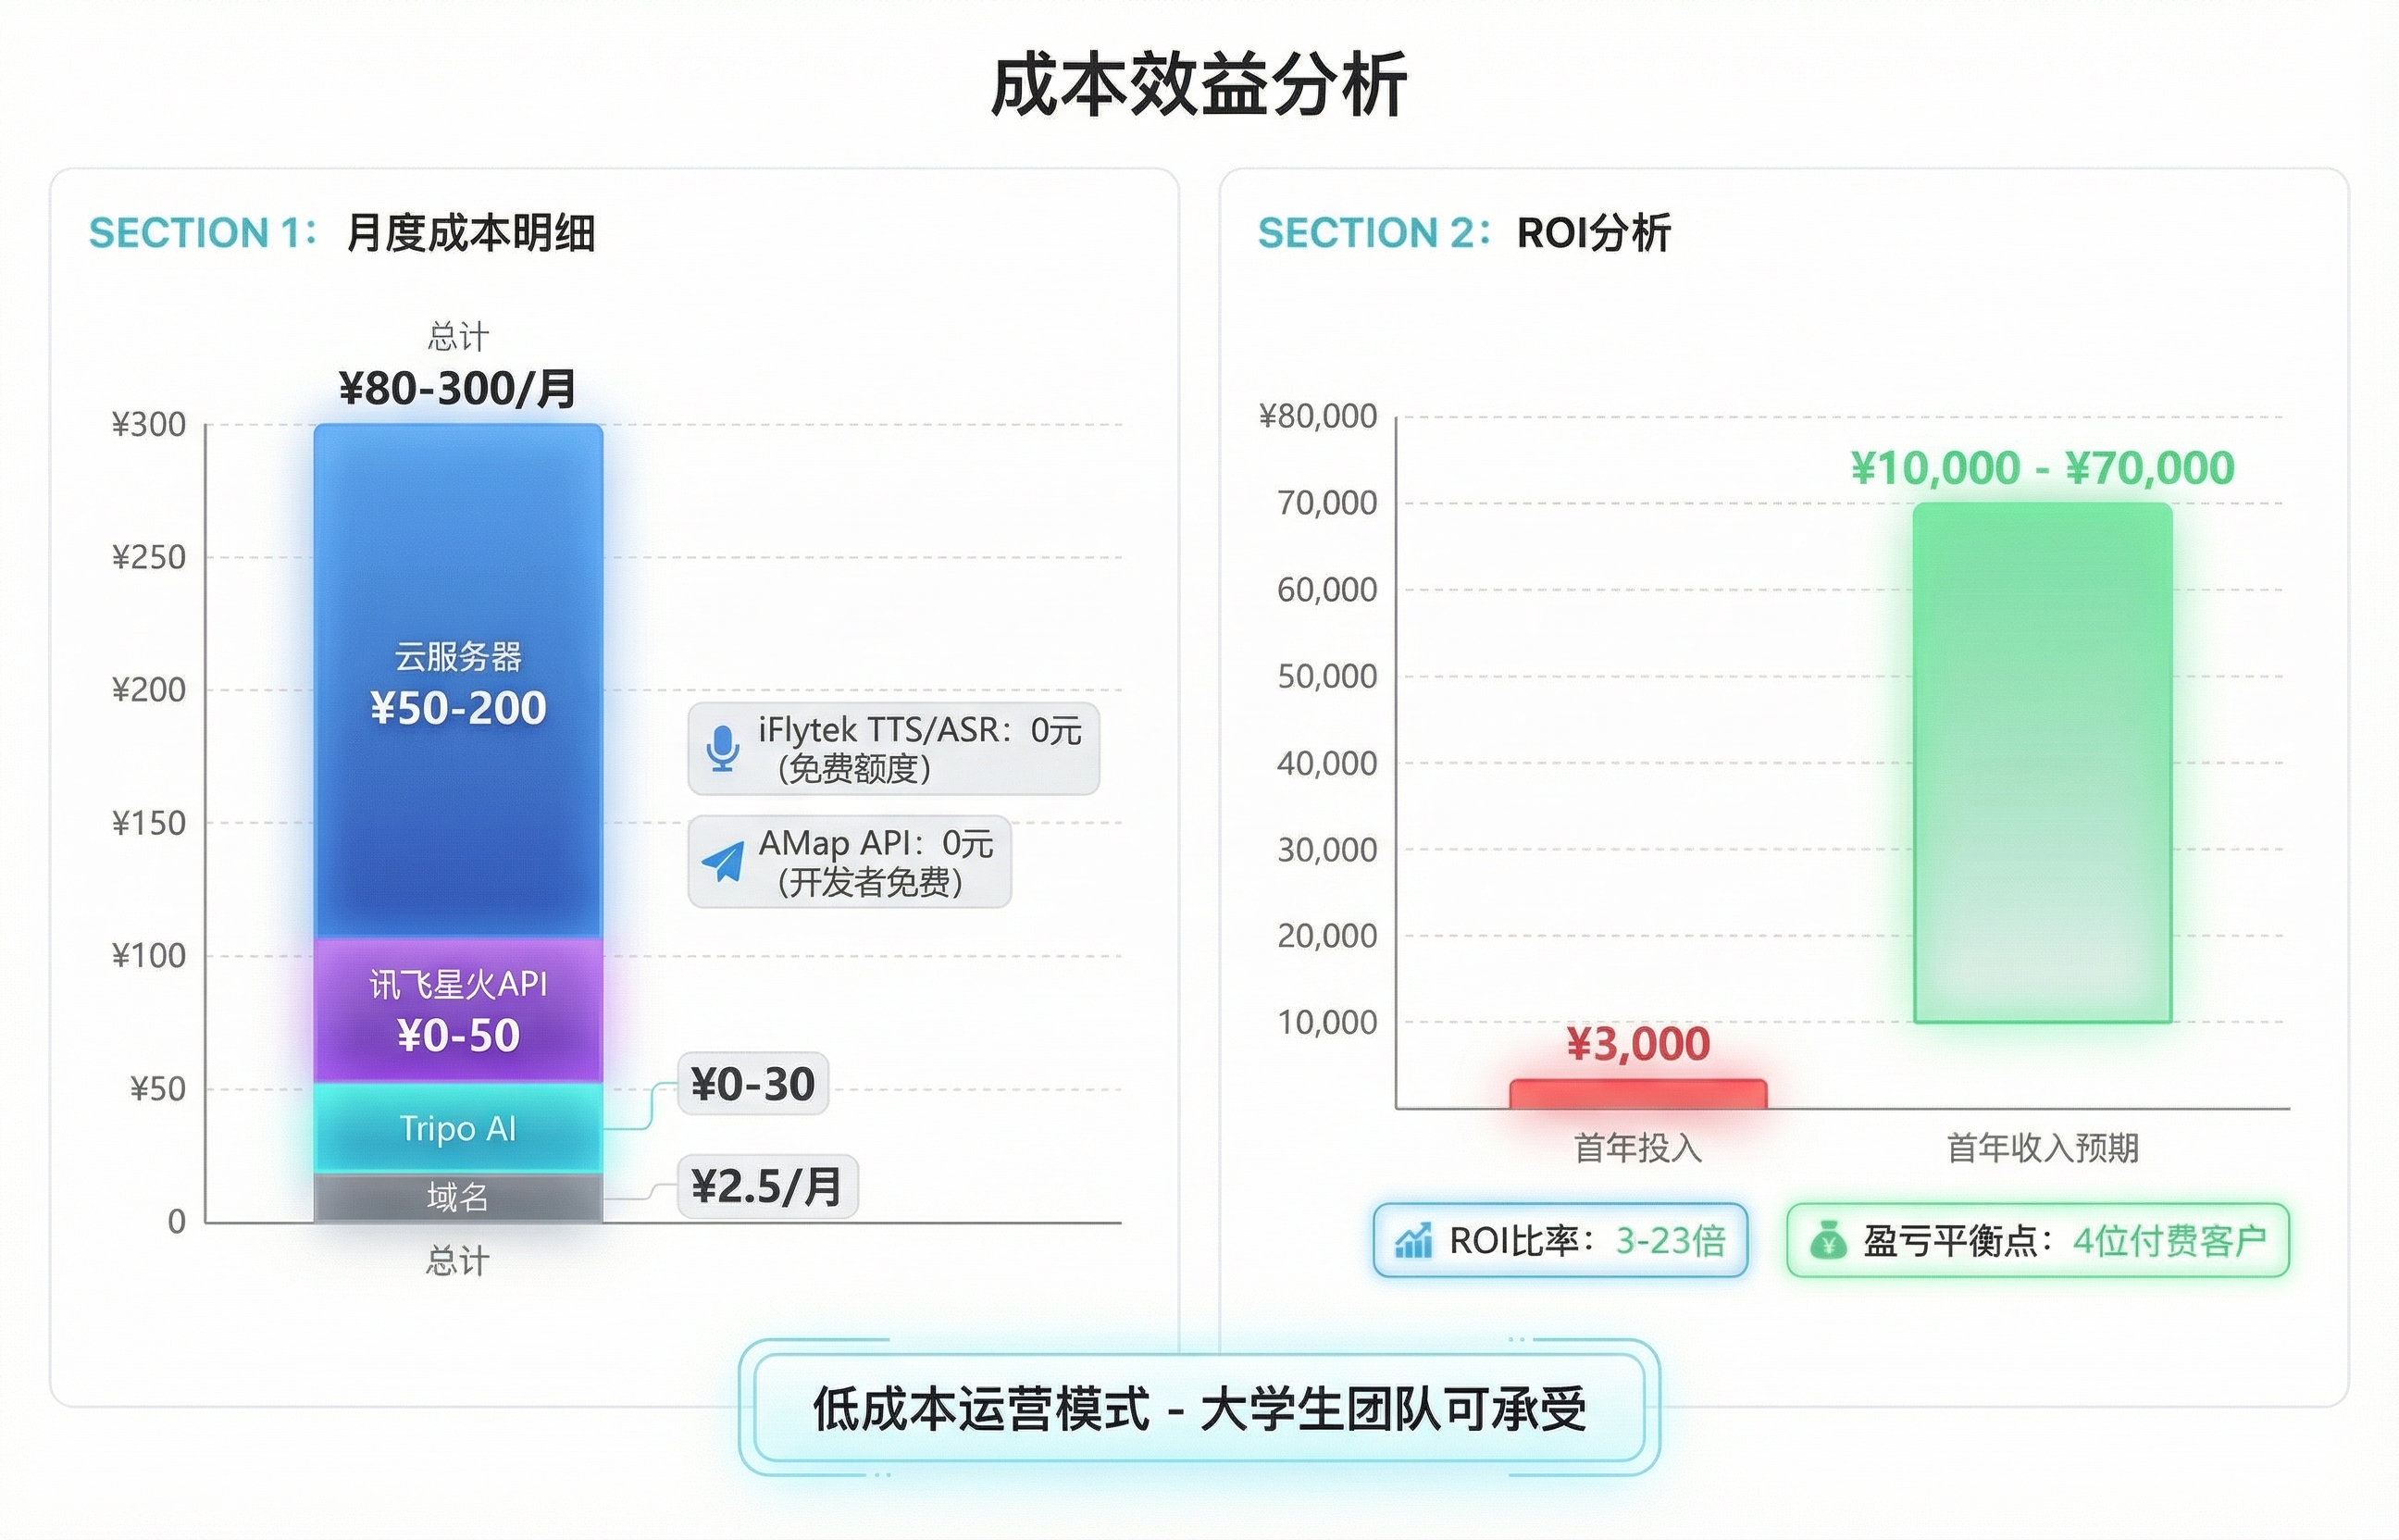
\includegraphics[width=0.85\textwidth]{../picture/fig13_cost_benefit.png}
\caption{成本收益分析图}
\end{figure}
